\documentclass[12pt]{beamer}

\usepackage[T1]{fontenc}
\usepackage[utf8]{inputenc}
\usepackage[portuguese, onelanguage]{algorithm2e}
\usepackage{amsmath, graphicx, hyperref, mathtools, subcaption, tikz-qtree}

\usetikzlibrary{positioning, matrix, arrows, decorations.markings}

\usetheme{CambridgeUS}
\usecolortheme{seagull}
\setbeamertemplate{title page}[default][shadow=false]
\setbeamertemplate{headline}{}
\setbeamertemplate{itemize items}[triangle]
\setbeamertemplate{footline}[frame number]{}
\setbeamertemplate{navigation symbols}{}

\title{Esquemas de assinatura digital \\ pós-quânticos baseados em AES}
\author{Gustavo Zambonin\and Marcello Klingelfus}
\institute{
  
\includegraphics[scale=0.15]{img/ufsc}        \\ \vspace{-4mm}
  Universidade Federal de Santa Catarina        \\
  Departmento de Informática e Estatística      \\ 
  INE5424 -- Sistemas Operacionais II           \\ \vspace{2mm}
  \texttt{\{gustavo.zambonin,marcello.klingelfus\}@grad.ufsc.br}
}
\date{}

\newcommand{\hh}{\mathcal{H}}
\newcommand{\pk}{\mathcal{P}_k}
\newcommand{\sk}{\mathcal{S}_k}
\newcommand{\hash}[2][]{\mathcal{H}^{#1}(#2)}
\newcommand{\concat}{\, \vert \vert \,}
\newcommand{\binwds}[1]{\{0, 1\}^{#1}}
\newcommand{\length}[1]{\vert #1 \vert}
\newcommand{\fhash}[1]{\hh{} : \binwds{*} \longrightarrow \binwds{#1}}

\tikzset{
  XOR/.style={draw,circle,append after command={
    [shorten >=\pgflinewidth, shorten <=\pgflinewidth,]
    (\tikzlastnode.north) edge (\tikzlastnode.south)
    (\tikzlastnode.east) edge (\tikzlastnode.west)}},
  edge/.style={->},
}

\begin{document}

\begin{frame}[plain,noframenumbering]
  \titlepage
\end{frame}

\begin{frame}
  \frametitle{Motivação}
  \begin{itemize}
    \setlength\itemsep{0.5em}
    \item Segurança de esquemas de assinatura digital é baseada em teoria de números ou problemas algébricos
    \begin{itemize}
      \item Insuficiente no âmbito de computadores quânticos
      \item Criptografia pós-quântica é independente destes problemas
    \end{itemize}
    \item Funções de mão única são necessárias e suficientes para assinatura digital~\cite{Rompel:1990:OFN:100216.100269}
    \begin{itemize}
      \item Base teórica de funções de resumo criptográfico
      \item Livre escolha, critério situacional (hardware, software)
      \item Cifras de bloco são utilizadas em sua construção~\cite[Sec. 9.14]{Menezes:1996:HAC:548089}
    \end{itemize}
  \end{itemize}
\end{frame}

\begin{frame}
    \frametitle{AES}
    \framesubtitle{Definições I}
    \begin{itemize}
        \item Versão padronizada pelo NIST do algoritmo Rjindael \cite{Daemen:2002:DR:560131}
        \begin{itemize}
            \item Principais escolhas de design: inversibilidade e eficiência
        \end{itemize}
        \item Cifra de blocos iterativa parametrizada por uma chave $K$
        \begin{itemize}
            \item Conceito de rede de substituição-permutação (\href{https://www.iacr.org/authors/tikz/tikz/Construction/spn.pdf}{SPN})
            \item $\length{K} \in \{128, 192, 256\}$
            \item 10, 12 ou 14 rodadas ($n_r$), respectivamente

            \item Deslocamentos de linhas e permutas de elementos
        \end{itemize}
    \end{itemize}
\end{frame}

\begin{frame}
    \frametitle{AES}
    \framesubtitle{Definições II}
    \begin{itemize}
        \item Opera sobre uma matriz de estado $A$, $A_{i,j} \in \mathbb{F}_{2^8}, 0 \leq i, j \leq 3$
        \begin{itemize}
            \item Para uma mensagem $m$ de $\length{K}$ bits, $A_{i,j} = m_{i+4j}$
        \end{itemize}
        \item Operações sobre bytes análogas a cálculos em $\mathbb{F}_{2^8}$
        \begin{itemize}
            \item Adição equivalente a $\oplus$
            \item Multiplicação usual, módulo o polinômio irredutível $x^8 + x^4 + x^3 + x + 1$
        \end{itemize}
        \begin{equation*}
            \begin{smallmatrix}
            E & P & O & S \\
            \end{smallmatrix}
        \end{equation*}
    \end{itemize}
\end{frame}

\begin{frame}
    \frametitle{AES}
    \framesubtitle{Etapa \emph{SubBytes}}
    \begin{columns}[T]
        \begin{column}{.7\textwidth}
          \begin{itemize}
                \item Caixa de substituição (\emph{S-box}) aplicada em cada $A_{i,j}$ individualmente
                \item Única etapa não-linear da cifra
                \item Transformação afim sobre $a = A^{-1}_{i,j}$
                    \begin{equation*}
                        A'_{i,j} = 
                        \begin{smallmatrix}
                        1 & 0 & 0 & 0 & 1 & 1 & 1 & 1 \\
                        1 & 1 & 0 & 0 & 0 & 1 & 1 & 1 \\
                        1 & 1 & 1 & 0 & 0 & 0 & 1 & 1 \\
                        1 & 1 & 1 & 1 & 0 & 0 & 0 & 1 \\
                        1 & 1 & 1 & 1 & 1 & 0 & 0 & 0 \\
                        0 & 1 & 1 & 1 & 1 & 1 & 0 & 0 \\
                        0 & 0 & 1 & 1 & 1 & 1 & 1 & 0 \\
                        0 & 0 & 0 & 1 & 1 & 1 & 1 & 1 \\
                        \end{smallmatrix} \cdot
                        \begin{smallmatrix}
                        a_0 \\ a_1 \\ a_2 \\ a_3 \\ a_4 \\ a_5 \\ a_6 \\ a_7 \\
                        \end{smallmatrix} +
                        \begin{smallmatrix}
                        1 \\ 1 \\ 0 \\ 0 \\ 0 \\ 1 \\ 1 \\ 0 \\
                        \end{smallmatrix}
                    \end{equation*}
                \item \emph{InvSubBytes}: inversa da transformação afim
            \end{itemize}
        \end{column}
        \begin{column}{.25\textwidth}
            \begin{figure}
            \centering
            \begin{subfigure}[b]{0.7\textwidth}
               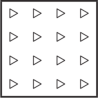
\includegraphics{img/sub_bytes_fwd.pdf}
               \vspace{2mm}
            \end{subfigure}
            
            \begin{subfigure}[b]{0.7\textwidth}
               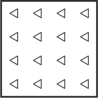
\includegraphics{img/sub_bytes_inv.pdf}
            \end{subfigure}
                    \captionsetup{font=scriptsize}
        
            \caption*{Pictogramas para as etapas \emph{SubBytes} (acima) e sua inversa \emph{InvSubBytes}.}
            \end{figure}
        \end{column}
    \end{columns}
\end{frame}

\begin{frame}
    \frametitle{AES}
    \framesubtitle{Etapa \emph{ShiftRows}}
    \begin{columns}[T]
        \begin{column}{.7\textwidth}
          \begin{itemize}
            \item Rotacionamento cíclico das linhas de $A$
            \item Provê difusão, impede que a cifra aja separadamente sobre as linhas
            \begin{equation*}
                \begin{matrix}
                    a & b & c & d \\
                    e & f & g & h \\
                    i & j & k & l \\
                    m & n & o & p \\
                \end{matrix} \; \longrightarrow \;
                \begin{matrix}
                    a & b & c & d \\
                    f & g & h & e \\
                    k & l & i & j \\
                    p & m & n & o \\
                \end{matrix}
            \end{equation*}
            \item \emph{InvShiftRows}: rotacionamento inverso
          \end{itemize}
        \end{column}
        \begin{column}{.25\textwidth}
            \begin{figure}
            \centering
            \begin{subfigure}[b]{0.7\textwidth}
               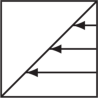
\includegraphics{img/shift_rows_fwd.pdf}
               \vspace{2mm}
            \end{subfigure}
            
            \begin{subfigure}[b]{0.7\textwidth}
               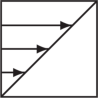
\includegraphics{img/shift_rows_inv.pdf}
            \end{subfigure}
                    \captionsetup{font=scriptsize}
        
            \caption*{Pictogramas para as etapas \emph{ShiftRows} (acima) e sua inversa \emph{InvShiftRows}.}
            \end{figure}
        \end{column}
    \end{columns}
\end{frame}

\begin{frame}
    \frametitle{AES}
    \framesubtitle{Etapa \emph{MixColumns}}
    \begin{columns}[T]
        \begin{column}{.7\textwidth}
          \begin{itemize}
            \item Permutação operando em cada coluna de $A$, também provendo difusão
            \item $a = A_j$ tratada como um polinômio e multiplicada por uma constante
            \begin{multline*}
                a' = (a_3 x^3 + a_2 x^2 + a_1 x^1 + a_0 x^0) \\
                \cdot (3 x^3 + x^2 + x + 2) \pmod{x^4 + 1}
            \end{multline*}
            \item \emph{InvMixColumns}: multiplicação por $(3 x^3 + x^2 + x + 2)^{-1}$
          \end{itemize}
        \end{column}
        \begin{column}{.25\textwidth}
            \begin{figure}
            \centering
            \begin{subfigure}[b]{0.7\textwidth}
               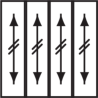
\includegraphics{img/mix_columns_fwd.pdf}
               \vspace{2mm}
            \end{subfigure}
            
            \begin{subfigure}[b]{0.7\textwidth}
               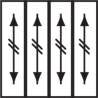
\includegraphics{img/mix_columns_inv.pdf}
            \end{subfigure}
                    \captionsetup{font=scriptsize}
        
            \caption*{Pictogramas para as etapas \emph{MixColumns} (acima) e sua inversa \emph{InvMixColumns}.}
            \end{figure}
        \end{column}
    \end{columns}
\end{frame}

\begin{frame}
    \frametitle{AES}
    \framesubtitle{Rotina \emph{KeyExpansion} e etapa \emph{AddRoundKey}}
          \begin{itemize}
            \item \emph{KeyExpansion}: chave expandida $K^e$, $\ell = \frac{\length{K}}{32}$ palavras por rodada
            \item ``\emph{Round constants}'':
                $RC_0 = x^0, RC_1 = x^1, RC_j = x^{j-1} \cdot RC_{j-1}, j > 2$
        
                $$K^e = (\overbrace{k_0, \dots, k_{\ell - 1}}^{K}, k_{\ell}, \dots, k_{(n_r + 1) \cdot \ell - 1})$$
                \begin{equation*}
  k_i = k_{i - \ell} + 
    \begin{cases}
      \textsc{SubBytes}(k_{i - 1} \stackrel{\curvearrowright}{\ll} 8) + RC_{\frac{i}{\ell}},
        \text{ se } i \equiv 0 \pmod{4} \\
      \textsc{SubBytes}(k_{i - 1}),
        \text{ se } \ell = 8 \text { e } i \equiv 4 \pmod{8} \\
      k_{i - 1}, \text{ caso contrário.}
    \end{cases}
\end{equation*}
        \item \emph{AddRoundKey}: $A' = A + (k_{\ell \cdot i}, \dots, k_{\ell \cdot (i + 1) - 1}), 0 \leq i \leq n_r$
          \end{itemize}
\end{frame}

\begin{frame}
    \frametitle{AES}
    \framesubtitle{Representação gráfica da codificação e decodificação para $n_r = 2$}
    \begin{figure}
        \centering
        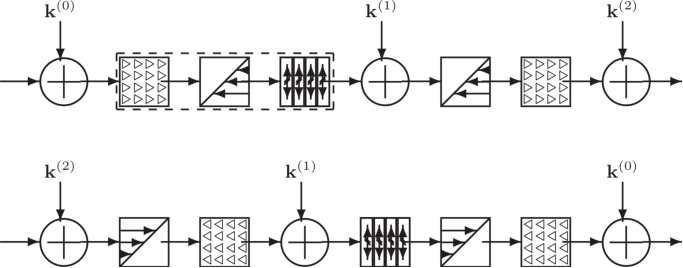
\includegraphics{img/aes_two_rounds.pdf}
        \label{fig:my_label}
    \end{figure}
\end{frame}

\begin{frame}
  \frametitle{Funções de resumo criptográfico}
  \begin{equation*}
    \mathcal{H}: \{0, 1\}^{*} \longrightarrow \{0, 1\}^{n}
  \end{equation*}

  \begin{figure}
    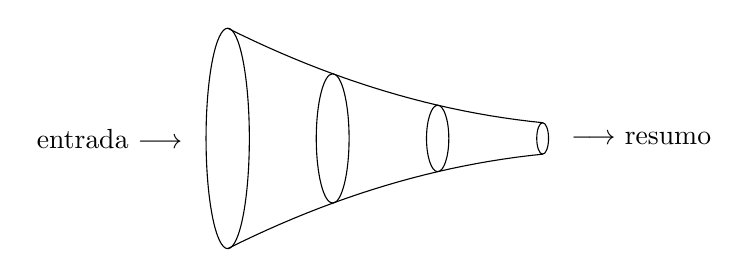
\begin{tikzpicture}
      \node at (-6.5, 0) {entrada $\longrightarrow$};
      \foreach \sgn in {+, -}
        \draw plot[domain=1:5] (-\x, {\sgn 1/20*(3+\x*\x)});
      \foreach \r in {1, 2.3333, ..., 5}
        \draw (-\r, 0) ellipse[x radius=(\r+.5)/20, y radius=1/20*(3+\r*\r)];
      \node at (0.25, 0) {$\longrightarrow$ resumo};
    \end{tikzpicture}
  \end{figure}

  \begin{itemize}
    \item SHA-2, SHA-3, BLAKE: $n \in \{224, 256, 384, 512\}$
    \item Keccak: qualquer $n$
    \item Resistência à pré-imagem, segunda pré-imagem, colisão
  \end{itemize}
\end{frame}

\begin{frame}
  \frametitle{Assinatura digital}
  \begin{itemize}
    \item Provê autenticação, integridade e não-repúdio
    \item Baseado em criptografia de chaves públicas
    \item Tripla de algoritmos probabilísticos de tempo polinomial
      \cite{Goldreich:2004:FCV:975541}
    \begin{itemize}
      \item Geração de chaves (\emph{Gen}), geração da assinatura (\emph{Sig}),\\
          verificação da assinatura (\emph{Ver})
    \end{itemize}
  \end{itemize}

    \begin{figure}[ht]
      \centering
      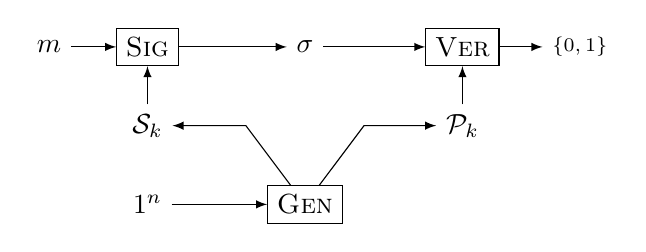
\begin{tikzpicture}
        \node (hm) at (-1.25, 0) {$m$};
        \node (in) at (0, -2) {$1^n$};
        \node (sk) at (0, -1) {$\sk{}$};
        \node (pk) at (4, -1) {$\pk{}$};
        \node (ds) at (2, 0) {$\sigma$};
        \node (res) at (5.5, 0) {\scriptsize $\binwds{}$};
        \node[draw] (sig) at (0, 0) {\textsc{Sig}};
        \node[draw] (gen) at (2, -2) {\textsc{Gen}};
        \node[draw] (ver) at (4, 0) {\textsc{Ver}};
        \draw[-latex] (gen) to (1.25, -1) to (sk);
        \draw[-latex] (gen) to (2.75, -1) to (pk);
        \draw[-latex] (sk) -- (sig);
        \draw[-latex] (hm) -- (sig);
        \draw[-latex] (sig) -- (ds);
        \draw[-latex] (ds) -- (ver);
        \draw[-latex] (pk) -- (ver);
        \draw[-latex] (ver) -- (res);
        \draw[-latex] (in) -- (gen);
      \end{tikzpicture}
    \end{figure}
\end{frame}

\begin{frame}
  \frametitle{Esquemas de assinatura única}
  \begin{itemize}
    \item Par de chaves só deve ser utilizado uma única vez
    \item Lamport-Diffie (LD-OTS)
    \begin{itemize}
      \item Primeiro esquema baseado em resumos
      \item Mensagens de tamanho arbitrário podem ser assinadas, um bit por vez
    \end{itemize}
    \item Winternitz (WOTS)
    \begin{itemize}
      \item Múltiplos bits podem ser assinados simultaneamente
      \item Generalização do LD-OTS
      \item Compensação entre desempenho e tamanho da assinatura
    \end{itemize}
  \end{itemize}
\end{frame}

\begin{frame}
  \frametitle{Winternitz OTS}
  \framesubtitle{Geração de chave}
  Seja $w \in \mathbb{N}, w > 1$ o parâmetro Winternitz,
  $f : \{0, 1\}^{n} \longrightarrow \{0, 1\}^{n}$
  e $\mathcal{H} : \{0, 1\}^{*} \longrightarrow \{0, 1\}^{n}$. Então,
   \begin{align*}
       t_1 &= \left\lceil \frac{n}{w} \right\rceil, t_2 = \left\lceil
       \frac{\lfloor log_2 t_1 \rfloor + 1 + w}{w} \right\rceil \text{ e } t = t_1 + t_2.
   \end{align*}
   As chaves privada e pública são, respectivamente,
   \begin{align*}
      \sk{} &= (y_{t - 1}, \dots, y_{0})
        \stackrel{\$}{\longleftarrow} \{0,1\}^n \text{ e}\\
      \pk{} &= (f^{2^w - 1}(y_{t - 1}), \dots, f^{2^w - 1}(y_0)).
   \end{align*}
\end{frame}

\begin{frame}
  \frametitle{Winternitz OTS}
  \framesubtitle{Assinatura}
  Os valores $\epsilon_i \in \{0, 1\}^w$ são obtidos através de:
  
  \begin{minipage}{.45\linewidth}
  \begin{align*}
    \mathcal{H}(m) &= (\epsilon_{t - 1}, \dots, \epsilon_{t - t_1})
  \end{align*}
  \end{minipage}
  \begin{minipage}{.45\linewidth}
  \begin{align*}
    c &= \sum_{i = t - t_1}^{t - 1} (2^w - 1 - \epsilon_i) \\
      &= (\epsilon_{t_2 - 1}, \dots, \epsilon_{0})
  \end{align*}
  \end{minipage}
  \vspace{4mm}
  
  Finalmente, a assinatura de uso único é construída:
  \begin{align*}
    \sigma &= (f^{\epsilon_{t - 1}}(y_{t - 1}), \dots, f^{\epsilon_0}(y_0))
  \end{align*}
\end{frame}

\begin{frame}
  \frametitle{Winternitz OTS}
  \framesubtitle{Verificação}
  Relembrando,
  \begin{align*}
    \pk{} &= (f^{2^w - 1}(y_{t - 1}), \dots, f^{2^w - 1}(y_0)) \text{ e} \\
    \sigma &= (f^{\epsilon_{t - 1}}(y_{t - 1}), \dots, f^{\epsilon_0}(y_0)).
  \end{align*}
  Os elementos $\epsilon_i$ são calculados e utilizados na verificação de $\sigma$:
  \begin{align*}
    \forall \sigma_i \in \sigma, f^{2^w - 1 - \epsilon_{i}}(\sigma_i) &= \mathcal{P}_{k_i}
  \end{align*}
  Resumidamente,
  \begin{figure}[ht]
  \centering
  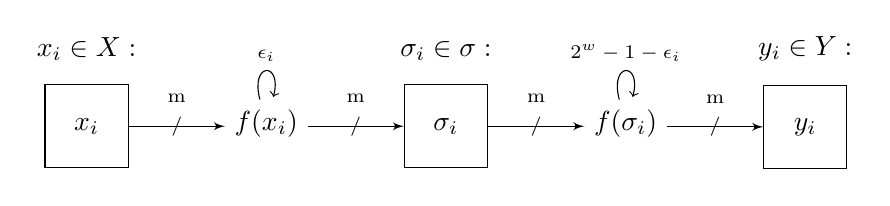
\begin{tikzpicture}[
    decoration={
      markings,
      mark= at position 0.5 with {\node[font=\scriptsize] {/};},
      mark= at position 0.5 with {\node[font=\scriptsize, yshift=10pt] {m};}
    }]
	\tikzstyle{arrowline}=[draw, -latex']
	\tikzstyle{abox}=[draw, minimum width=30pt, minimum height=30pt]

    \matrix[matrix of nodes, column sep=35pt, row sep=30pt, ampersand replacement=\&] {
		\node [abox] (xt1) {$x_i$}; \&
		\node (fst1) {$f(x_i)$}; \&
		\node [abox] (st1) {$\sigma_i$}; \&
		\node (fvt1) {$f(\sigma_i)$}; \&
		\node [abox] (yt1) {$y_i$}; \\
    };

	\node[above = 5pt of xt1] (X) {$x_i \in X:$};
	\node[above = 5pt of st1] (S) {$\sigma_i \in \sigma:$};
	\node[above = 5pt of yt1] (Y) {$y_i \in Y:$};

 	\path[arrowline, postaction={decorate}] (xt1)      --      (xt1 -| fst1.west);
 	\path[arrowline, postaction={decorate}] (fst1.east |- st1)      --      (st1);
    \path[->] (fst1) edge  [loop above] node {\scriptsize$\epsilon_i$} ();
 	\path[arrowline, postaction={decorate}] (st1)      --      (st1 -| fvt1.west);
 	\path[arrowline, postaction={decorate}] (fvt1.east |- yt1)      --      (yt1);
    \path[->] (fvt1) edge  [loop above] node {\scriptsize$2^w - 1 - \epsilon_i$} ();
  \end{tikzpicture}
\end{figure}
\end{frame}

\begin{frame}
  \frametitle{Winternitz OTS}
  \framesubtitle{Variante WOTS+}
  \begin{itemize}
    \item Elimina a necessidade de $\hh{}$ resistente a colisões
    \begin{itemize}
      \item Modificação da função de iteração $f$ para uma família
      $\mathcal{F}_k : \{f_k : \binwds{n} \longrightarrow \binwds{n} \mid k \in \mathcal{K}_n\}$
    \end{itemize}
    \item Máscaras de bits aleatórias em cada iteração
    \begin{align*}
      r &= (r_0, \dots, r_{2^w - 1}) \stackrel{\$}{\longleftarrow} \binwds{n} \\
      c^{0}_{k}(x, r) &= x \\
      c^{i}_{k}(x, r) &= f_k(c^{i-1}_{k}(x, r) \oplus r_i).
    \end{align*}
    \item Derivação de $f$ a partir de uma cifra de bloco
  \end{itemize}
\end{frame}

\begin{frame}
  \frametitle{Winternitz OTS}
  \framesubtitle{Utilizando AES como $f_k$ em WOTS+}
  \begin{itemize}
      \item Construção Matyas-Meyer-Oseas \cite[Sec. 9.41]{Menezes:1996:HAC:548089}
      \begin{itemize}
        \item Tome uma cifra $E_K$ com bloco de $n$ bits
        \item Divida a entrada em $k$ blocos de $n$ bits, $X = (x_0, \dots, x_{k - 1})$
        \item Tome um valor inicial $IV$ e uma função $g$ que gere chaves válidas para $E$
        \item $h_0 = IV, h_i = E_{g(h_{i-1})}(x_i) \oplus x_i, 1 \leq i \leq k$
      \end{itemize}
  \end{itemize}
  \begin{figure}[ht]
  \centering
  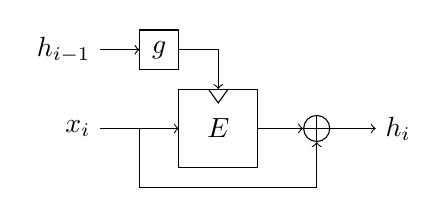
\begin{tikzpicture}[scale=0.25]
    \draw (-2, 5) rectangle node {$g$} ++(2, 2);
    \draw (0, 0) rectangle node {$E$} ++(4, 4);
    \draw (1.5, 4) -- ++(0.5,-0.7) -- ++(0.5, +0.7);
    \node[XOR] (x0) at (7,2) {};
    \draw[edge] (-4,2) node[left] {$x_{i}$} -- ++(4,0);
    \draw[edge] (4,2) -- (x0);
    \draw[edge] (x0) -- ++(3,0) node[right] {$h_{i}$};
    \draw[edge] (-2,2) -- ++(0,-3) -- ++(9,0) -- (x0);
    \draw[edge] (-4,6) node[left] {$h_{i-1}$} -- ++(2, 0);
    \draw[edge] (0, 6) -- ++(2, 0) -- ++(0, -2);
  \end{tikzpicture}
\end{figure}
\end{frame}

\begin{frame}
  \frametitle{Esquemas baseados em árvores de Merkle}
  \begin{columns}[T]
    \begin{column}{.4\textwidth}
      \begin{itemize}
        \item Assinaturas únicas em cada folha, árvore construída a partir de chaves públicas
        \item Estado da arte dos esquemas baseados em funções de resumo criptográfico
        \item XMSS, XMSS$^{MT}$, SPHINCS
      \end{itemize}
    \end{column}
    \begin{column}{.4\textwidth}
      \begin{figure}[ht]
  \centering
  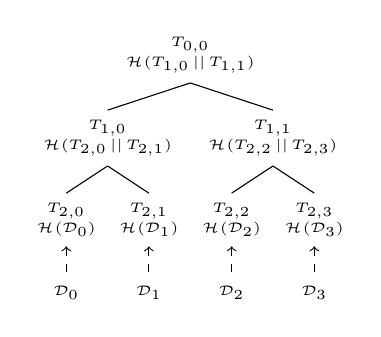
\begin{tikzpicture}
    \tikzset{every tree node/.style={align=center,anchor=north,font=\tiny}}
    \Tree
      [.\node{$T_{0,0}$ \\ $\hash{T_{1,0} \concat T_{1,1}}$};
        [.\node{$T_{1, 0}$ \\ $\hash{T_{2, 0} \concat T_{2, 1}}$};
          [.{$T_{2, 0}$ \\ $\hash{\mathcal{D}_{0}}$}
            \edge[dashed, style={<-}] node {}; $\mathcal{D}_{0}$
          ]
          [.{$T_{2, 1}$ \\ $\hash{\mathcal{D}_{1}}$}
            \edge[dashed, style={<-}] node {}; $\mathcal{D}_{1}$
          ]
        ]
        [.\node{$T_{1, 1}$ \\ $\hash{T_{2, 2} \concat T_{2, 3}}$};
          [.{$T_{2, 2}$ \\ $\hash{\mathcal{D}_{2}}$}
            \edge[dashed, style={<-}] node {}; $\mathcal{D}_{2}$
          ]
          [.{$T_{2, 3}$ \\ $\hash{\mathcal{D}_{3}}$}
            \edge[dashed, style={<-}] node {}; $\mathcal{D}_{3}$
          ]
        ]
      ]
  \end{tikzpicture}
        \captionsetup{font=scriptsize}
        \caption*{Seja $\mathcal{D}_n$ um dado qualquer. Uma árvore de Merkle é construída recursivamente através da concatenação dos resumos dos filhos de um nó.}
      \end{figure}
    \end{column}
  \end{columns}
\end{frame}

\begin{frame}[allowframebreaks]
  \frametitle{Bibliografia}
  \bibliographystyle{apalike}
  \bibliography{report}
\end{frame}

\end{document}
